%preambulo
\documentclass[]{beamer}
\usepackage[spanish]{babel}
\usepackage[utf8]{inputenc}

%justificado
\usepackage{ragged2e}
\justifying

%tema
\usetheme{Warsaw}
\usecolortheme{default}
\setbeamercovered{transparent}

\title [Ingeniería en Software]{Personal Software Process - ISO/IEC 12207}
\author[Grupo 1]{Oscar León Trureo\\Sebastián Menéndez Sáez\\Claudio Piña Novoa}
\date{\today}
\institute[]{Universidad Tecnol\'ogica Metropolitana}
%\logo{}


%empieza el Documento
\begin{document}


\begin{frame}
	\maketitle
\end{frame}

\begin{frame}
	\frametitle{Índice}
	\tableofcontents[]
\end{frame}

\section{Personal Software Process}
		\subsection{Introducci\'on}
			\begin{frame}{Introducci\'on}
				Dentro del mundo del desarrollo en Software, podemos encontrar las metodolog\'ias, las cuales son un conjunto de buenas pr\'acticas, las cuales nos permiten:\\ \pause
				\begin{itemize}
					\item Crear mejores aplicaciones.\pause
					\item Llevar un mejor proceso de desarrollo.\pause
					\item Agilizar el desarrollo en sí.\pause
					\item etc \ldots
				\end{itemize}				
			\end{frame}
			
			\begin{frame}{Introducci\'on}
				Existen una gran cantidad de metodologías, las cuales pueden estar enfocadas al desarrollo en sí, a la gestión, a la calidad, al desarrollador, como también puede ser una mezcla.\\
				\smallskip
				Personal Software Process, es una metodolog\'ia enfocada a la calidad del desarrollo del software a nivel personal, la cual se basa en factores que veremos más adelante.
			\end{frame}						
			
		\subsection{Historia}
			\begin{frame}{Historia}
				\pause
				\begin{itemize}
					\item Creado en el año 1995 por Watt's S. Humphrey en la Universidad de Carnegie Mellon, en Pittsburgh, Pennsylvania.\\ \pause
					\item El primer curso fue imparti\'o en la Universidad de Carnegie Mellon.\\ \pause
					\item fue plasmado en el libro ``A Discipline for SW Engineering'' de Humphrey.\\
				\end{itemize}
			\end{frame}
		
				\begin{frame}
					\begin{quotation}``La calidad del software está dada por la cantidad de procesos usados para desarrollarlo y mantenerlo''.\end{quotation}
			
				\hfill -- \parbox[t]{.9\textwidth}{Watts S. Humphrey,
				\textit{Creador de Personal Software Process}}

				\end{frame}
		
		\subsection{PSP}
			\begin{frame}{PSP}
				\textbf{Personal Software Process}, que en español significa \textbf{Proceso Personal de Software} (PSP), es un conjunto de buenas pr\'acticas las cuales se enfocan al control del tiempo y en la productividad de los Ingenieros en Software, ya sea en la mantencion de sistemas o en tareas de desarrollo.
			\end{frame}
			
			\begin{frame}{PSP}
				\textbf{PSP} no es un est\'andar, es m\'as bien un alternativa que permite mejorar la forma en la que se construye el software, pero con un enfoque ``individual'', por lo que es muy recomendada para los desarrolladores que estén interesados en mejorar en lo que llamamos ``desarrollo individual''.
				\begin{figure}
    				\scalebox{0.2}{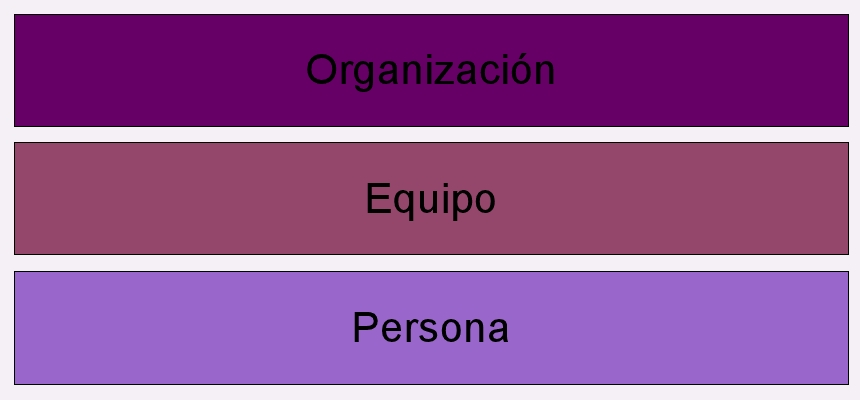
\includegraphics{Imagenes/Orga.jpg}} \caption{Niveles de la Organización}
				\end{figure}
			\end{frame}
				
			\begin{frame}{Pasos para la implementación de PSP}
				\begin{enumerate}
					\item Los ingenieros deben ser entrenados por un instructor calificado de PSP. \\ \smallskip \pause
					\item La Capacitacion es sobre grupos o equipos, y seran grupos que asi lo han sido y seguiran siendo. \\ \smallskip \pause
					\item Requiere un fuerte soporte de administración, en este sentido es necesario que los administradores entiendan el PSP, saber como apoyarlos y como monitorear sus avances, sin un adecuado monitoreo los ingenieros caeran otra vez en los malos habitos. \\ \smallskip \pause
					\item Después de ser bien entrenados y bien administrados lo que sigue es optimizar la interaccion entre equipos y aquí entraría Team Software Process, el TSP extiende y refina los metodos de CMM y PSP sobre desarrollo y mantenimiento de equipos, y llegar a lo que se le llama un equipo autodirigido. \\ \smallskip
				\end{enumerate}
			\end{frame}		
			
			\begin{frame}{Ciclo de Vida de PSP}
				Personal Software Process (PSP), tiene un ciclo de vida el cual consta de 7 fases, las cuales son fundamentales para el desarrollo de esta metodología: \\ \pause
				\begin{enumerate}
					\item Planeación \pause
					\item Diseño de Alto Nivel \pause
					\item Revisión de Alto Nivel \pause
					\item Desarrollo Ciclico \pause
					\item Post Mortem \pause
					\item Integración \pause
					\item Pruebas
				\end{enumerate}
			\end{frame}								
				
			\begin{frame}{Fase de Planeación}
				
			\end{frame}
\section{ISO/IEC 12207}
		\subsection{Introducci\'on}
			\begin{frame}{Introducci\'on}
				contenido introducción
			\end{frame}
		
		\subsection{Historia}
			\begin{frame}{Historia}
				contenido historia ISO
			\end{frame}
			
		\subsection{Desarrollo1}
			\begin{frame}{Desarrollo1}
				contenido Desarrollo1
			\end{frame}

		\subsection{Desarrollo2}
			\begin{frame}{Desarrollo2}
				contenido Desarrollo2
			\end{frame}
			
\section{Conclusi\'on}
	\begin{frame}{Conclusión}
		aqu\'i va la conclusi\'on
	\end{frame}				
			
\section{Bibliograf\'ia}
	\begin{frame}{Bibliograf\'ia}
		\begin{thebibliography}{9}
		
			%item 1		
			\bibitem{mo02} 
 			Victor M. Fleites Sabido 
 			\newblock {\em Personal Software Process}, 
 			\newblock http://www.slideshare.net/Tonymx/introduccion-a-personal-software-process.
		
			%item 2		
			\bibitem{sm-hin04} 
 			Armando David Espinoza Robles
 			\newblock{\em Metodologías de Desarrollo de Software}, 
 			\newblock http://www.slideshare.net/juliopari/4-clase-metodologia-de-desarrolo-de-software.
 			
		http://calidadesoftware.wordpress.com/2012/02/23/personal-software-process/ 			
		http://es.pdfsb.com/readonline/5a56464364516835575846394358706755554d3d-118608
 			
 		http://ingsw.ccbas.uaa.mx/sitio/images/material/psp.htm
		\end{thebibliography}
	\end{frame}

\end{document}